\documentclass{article}
% Package to manage page layout
\usepackage[margin=1.5cm, includefoot, footskip=30pt]{geometry}

\setlength\parindent{0pt}
\setlength{\parskip}{1em}

%%%%%%%PACKAGES HERE%%%%%%%
\usepackage{amsmath}
\usepackage{amsthm}
\usepackage{amssymb}
\usepackage{hyperref}
\usepackage{standalone}
\usepackage{subcaption}
\usepackage{tikz}
\usepackage{booktabs}
\usepackage{minted}
\usepackage{multicol,multirow,array}
\usepackage{algorithm,algorithmic}
\usetikzlibrary{er,positioning, calc, patterns}
\usetikzlibrary{decorations.pathreplacing}

\definecolor{background}{RGB}{5, 66, 81}
\usemintedstyle{tango}

\setcounter{secnumdepth}{4}
\setcounter{tocdepth}{4}

\usepackage{kbordermatrix}
\theoremstyle{definition}
\newtheorem{definition}{Definition}[section]

%%%%%%%%%%%%%%%%%%%%%%%%%%%%%%%PARAMETERS%%%%%%%%%%%%%%%%%%%%%%%%%%%%%%%%%%%%%%%
\newcommand{\totalarticles}{\input{assets/total_articles.txt}}
\newcommand{\uniquetitles}{\input{assets/unique_titles.txt}}
\newcommand{\numberofduplicates}{\input{assets/number_of_duplicates.txt}}
\newcommand{\manual}{\input{assets/prov_manual.txt}}
\newcommand{\authors}{\input{assets/authors.txt}}
\newcommand{\edges}{3174}
\newcommand{\auctionauthors}{\input{assets/authors_auction.txt}}
\newcommand{\auctionedges}{\input{assets/edges_auction.txt}}
\newcommand{\priceauthors}{\input{assets/authors_price.txt}}
\newcommand{\priceedges}{\input{assets/edges_price.txt}}
\newcommand{\prisonerscon}{\input{assets/prisoners_connected_components.txt}}
\newcommand{\prisonerscc}{\input{assets/prisoners_clustering.txt}}
\newcommand{\pricecon}{162}
\newcommand{\pricecc}{0.71}
\newcommand{\auctioncon}{\input{assets/auction_connected_components.txt}}
\newcommand{\auctioncc}{\input{assets/auction_clustering.txt}}
\newcommand{\prisonerisolated}{\input{assets/prisoners_isolated.txt}}
\newcommand{\auctionisolated}{\input{assets/auction_isolated.txt}}
\newcommand{\priceisolated}{\input{assets/price_isolated.txt}}
%%%%%%%%%%%%%%%%%%%%%%%%%%%%%%%%%%%%%%%%%%%%%%%%%%%%%%%%%%%%%%%%%%%%%%%%%%%%%%%%
%%%%%%%%%%%%%%%%%%%%%%%%%%%%%%%%%%%%%%%%%%%%%%%%%%%%%%%%%%%%%%%%%%%%%%%%%%%%%%%%
\title{A systematic literature review of the Prisoner's Dilemma; collaboration and influence.}
\author{Nikoleta E. Glynatsi, Vincent A. Knight}
\date{2016}

\begin{document}

\maketitle

\begin{abstract}
    The prisoner's dilemma is a well known game used since the 1950's as a framework
    for studying the emergence of cooperation; a topic of continuing interest
    for mathematical, social, biological and ecological sciences. The iterated version
    of the game attracted attention in the 1980's after
    the publication of the ``The Evolution of Cooperation'' and has been a topic
    of pioneering research ever since. This paper aims to provide a detailed
    literature review of the field. This is achieved by partitioning the timeline into six different
    sections. Furthermore, a comprehensive data set of literature is analysed
    using network theoretic approaches in order to explore the influence and the
    collaborative behaviour of the field itself.
\end{abstract}

\section{Introduction}\label{section:introduction}

In everyday life people choose between being selfish or being selfless when they
interact with others. The question that arises is: which behaviour is more beneficial?
There is a simple way of representing these behaviours/concepts. This is to use a
particular two player non-cooperative game called the prisoner's dilemma, originally
described in~\cite{Flood1958}.

Each player has two choices, to either be selfness and cooperate or to act in a
selfish manner and choose to defect. Each decision is made simultaneously and independently.
The fitness of each player is influenced by its own behaviour, and the behaviour
of the opponent. Both players do better if they choose to cooperate than if both
choose to defect. However, a player has the temptation to deviate as that player will
receive a higher payoff than that of a mutual cooperation.

A player's payoffs are generally represented by (\ref{eq:the_pd_payoffs}). Both
players receive a reward for mutual cooperation, \(R\), and a payoff \(P\) for
mutual defection. A player that defects while the other cooperates receives a payoff of
\(T\), whereas the cooperator receives \(S\). The dilemma exists due
to constrains (\ref{eq:constrain_one}) and (\ref{eq:constrain_two}).

\begin{equation} \label{eq:the_pd_payoffs}
    \begin{pmatrix}
    R & S \\ T & P
    \end{pmatrix}
\end{equation}

\begin{equation}\label{eq:constrain_one}
    T > R > P > S
\end{equation}

\begin{equation}\label{eq:constrain_two}
    2R > T + S
\end{equation}

Another common representation of the payoff matrix is given by~(\ref{eq:the_pd_payoffs_with_cost}),
where \(b\) is the benefit of the altruistic behaviour and \(c\) it's its cost
(constrains (\ref{eq:constrain_one}) - (\ref{eq:constrain_two}) still hold).

\begin{equation}\label{eq:the_pd_payoffs_with_cost}
    \begin{pmatrix}
        b - c & c \\ b & 0
    \end{pmatrix}
\end{equation}

Constrains (\ref{eq:constrain_one}) - (\ref{eq:constrain_two}) and rational behaviour
guarantee that it never benefits a player to cooperate. However,
when the game is studied in a manner where prior outcome matters,
defecting is no longer necessarily the dominant choice.

The repeated form of the game is called the iterated prisoner's dilemma and theoretical
works have shown that cooperation can emerge once players interact repeatedly.
Arguably, the most important of these works has been R. Axelrod's
``The Evolution of Cooperation''~\cite{Axelrod1984}.
In his book Axelrod reports on a series of computer tournaments he organised of
a finite turns games of the iterated prisoner's dilemma. Participants
had to choose between cooperation and defection again and again while having
memory of their previous encounters. Academics from several fields were invited to
design computer strategies to compete. The pioneering work of Axelrod
showed that greedy strategies did very poorly in the long run whereas altruistic
strategies did better.

``The Evolution of Cooperation'' is considered a milestone in the field but it
is not the only one. On the contrary, the prisoner's dilemma has attracted much
attention ever since the game's origins. In Section~\ref{section:analysis} a comprehensive
data set of literature regarding the prisoner's dilemma, and collected from
the following sources, is presented and analysed.

\begin{multicols}{2}
    \begin{itemize}
        \item arXiv~\cite{mckiernan2000}; a repository of electronic preprints.
        It consists of scientific
        papers in the fields of mathematics, physics, astronomy, electrical engineering,
        computer science, quantitative biology, statistics, and quantitative finance,
        which all can be accessed online.
        \item PLOS~\cite{plos}; a library of open access journals and other scientific literature
        under an open content license. It launched its first journal, PLOS Biology,
        in October 2003 and publishes seven journals, as of October 2015.
        \item IEEE Xplore Digital Library (IEEE)~\cite{ieee}; a research database for discovery
        and access to journal articles, conference proceedings, technical standards,
        and related materials on computer science, electrical engineering and electronics,
        and allied fields. It contains material published mainly by the Institute of
        Electrical and Electronics Engineers and other partner publishers. 
        \item Nature~\cite{nature}; a British multidisciplinary scientific journal,
        first published on 4 November 1869. It was ranked the world's most cited
        scientific journal by the Science Edition of the 2010 Journal Citation Reports
        and is ascribed an impact factor of 40.137, making it one of the world's
        top academic journals.
        \item Springer~\cite{springer}; a leading global scientific publisher of
        books and journals. It publishes close to 500 academic and professional
        society journals.
    \end{itemize}
\end{multicols}

The aim of the analysis is to review the amount of published academic articles
as well as to measure and explore the collaborations within the field.

\section{Timeline}\label{section:timeline}

In this section a large amount of literature regarding the prisoner's
dilemma is reviewed. The review starts from the year the game was formulated
and covers publications all the way to today.

\subsection{Origins of the prisoner's dilemma}\label{section:origin}

The origin of the prisoner's dilemma goes back to the 1950s in early experiments
conducted at RAND~\cite{Flood1958} to test the applicability of games
described in~\cite{VonNeumann1944}. The game received it's name later the same year.
According to~\cite{Tucker1983}, A. W. Tucker (the PhD supervisor of J. Nash~\cite{Nash1951}),
in an attempt to delivery the game with a story during a talk described the players
as prisoners and the game has been known as the prisoner's dilemma ever since.

The early research on the prisoner's dilemma had been very constrained. The only
source of experimental results was through groups of humans that simulated rounds
of the games and human groups came with disadvantages. Human can behave very
randomly and in several experiments both the size and the background of the
individuals were different. Thus comparing results of two or more studies
became tricky.

The main aim of these experiments had been to understand the conditions behind
the emergence of cooperation. Conditions such as the gender~\cite{Evans1966, Lutzker1961, Mack1971} of
individuals, the representation of the game~\cite{Evans1966}, the distance between
players~\cite{Sensenig1972}, the initial effects~\cite{Tedeschi1968} and whether
the experimenter was biased~\cite{Gallo1968} were being explored and still are
today.

An early figure that sought out to understand the conditions under which altruist
behaviour emerged was Prof A. Rapoport. A mathematical psychologist, whose work focused on
how to promote international and national cooperation. Rapoport tried to conceptualize
strategies that could promote international cooperation. In his teaching and research
he used the prisoner's dilemma. Rapoport offered the field many insights, he
is the creator of strategies such as Tit for Tat and Pavlov, which are going to be
discussed in later parts of this paper.

Decades later the political scientist R. Axelrod introduced the 
pioneer computer tournaments that have largely replaced human subjects in the study
of the iterated prisoner's dilemma ever since. In the next section  these
tournaments and several strategies that were design by researchers,
such as Rapoport, are introduced.

\subsection{Axelrod's tournaments and intelligent design of strategies}\label{subsection:intelligent_design}

As discussed in Section~\ref{section:origin}, before 1980 a great deal of
research was done in the field, however, as described in~\cite{Axelrod2012}, the
political scientist R. Axelrod believed that there was no clear answer to the question
of how to avoid conflict, or even how an individual should play the game. Combining
his interest in artificial intelligence and political sciences Axelrod created a
framework for exploring these questions using computer tournaments.

Axelrod's tournaments made the study of cooperation of critical interest
once again, academic articles were being published reproducing Axelord's work,
accessing and further developing his results. As described in~\cite{Rapoport2015},
``Axelrod's “new approach” has been extremely
successful and immensely influential in casting light on the conflict between an
individual and the collective rationality reflected in the choices of a population
whose members are unknown and its size unspecified, thereby opening a new avenue
of research''.
In a collaboration with a colleague, Douglas Dion, Axelrod in~\cite{Axelrod1988}
summarized a number of works that were immediately inspired from the ``Evolution of Cooperation''
and in 2012,~\cite{Jurisic2012} wrote a review on iterated prisoner's
dilemma strategies and big competitions that had occurred since the originals.

In essence, Axelrod asked researchers to design a strategy,
set a number of rules, with the purpose of wining an iterated prisoner's dilemma
tournament. These strategies were constructed by an intelligent cause and not an
undirected process, and here there are refereed to as strategies of intelligent
design. This section covers Axelrod's original tournaments as well as 
research that introduced new strategies of intelligent design.

The first reported computer tournament took place in 1980~\cite{Axelrod1980a}.
Several scientists were invited to submit their strategies, written in the
programming languages Fortran or Basic. There was a total of 13 submissions
made by the following researchers,

\begin{multicols}{2}
    \begin{enumerate}
        \item T Nicolaus Tideman and Paula Chieruzz;
        \item Rudy Nydegger;
        \item Bernard Grofman;
        \item Martin Shubik;
        \item Stein and Anatol Rapoport;
        \item James W Friedman;
        \item Morton Davis;
        \item Jim Graaskamp;
        \item Leslie Downing;
        \item Scott Feld;
        \item Johann Joss;
        \item Gordon Tullock;
    \end{enumerate}
\end{multicols}

and a \(13^{th}\) who remained anonymous.

Each competed in a 200 turn match against all 12 opponents, itself and a player
that played randomly (called \textbf{Random}). This type of tournament is referred to as a round robin.
The tournament was run only once, each participant knew
the exact length of the matches and had access to the full history of each match.
Furthermore, Axelrod performed a preliminary tournament and the results were known
to the participants. The payoff values used for equation~(\ref{eq:the_pd_payoffs}) where
\(R=3, P=1, T=5\) and \(S=0\). These values are commonly used in the literature
and unless specified will be the values used in the rest of the work described here.

The winner of the tournament was determined by the total average score and not by
the number of matches won. The strategy that was announced the winner was
submitted by Rapoport and was called \textbf{Tit For Tat}. Tit for Tat, is a
strategy that always cooperates on the first round and then mimics the opponent's
previous move.
The success of Tit for Tat came as a surprise. It was not only the simplest submitted
strategy but it had also won the tournament even though it could never do better
than any player it was interacting with.

In order to further test the results Axelrod performed a second
tournament later in 1980~\cite{Axelrod1980b}. The results of the first tournament
had been publicised and the second tournament received much more attention, with 62 entries
made by the following people,

\begin{multicols}{3}
    \begin{enumerate}
        \item Gail Grisell;
        \item Harold Rabbie;
        \item James W Friedman;
        \item Abraham Getzler;
        \item Roger Hotz;
        \item George Lefevre;
        \item Nelson Weiderman;
        \item Tom Almy;
        \item Robert Adams;
        \item Herb Weiner;
        \item Otto Borufsen;
        \item R D Anderson;
        \item William Adams;
        \item Michael F McGurrin;
        \item Graham J Eatherley;
        \item Richard Hufford;
        \item George Hufford;
        \item Rob Cave;
        \item Rik Smoody;
        \item John Willaim Colbert;
        \item David A Smith;
        \item Henry Nussbacher;
        \item William H Robertson;
        \item Steve Newman;
        \item Stanley F Quayle;
        \item Rudy Nydegger;
        \item Glen Rowsam;
        \item Leslie Downing;
        \item Jim Graaskamp and Ken Katzen;
        \item Danny C Champion;
        \item Howard R Hollander;
        \item George Duisman;
        \item Brian Yamachi;
        \item Mark F Batell;
        \item Ray Mikkelson;
        \item Craig Feathers;
        \item Fransois Leyvraz;
        \item Johann Joss;
        \item Robert Pebly;
        \item James E Hall;
        \item Edward C White Jr;
        \item George Zimmerman;
        \item Edward Friedland;
        \item X	Edward Friedland;
        \item Paul D Harrington;
        \item David Gladstein;
        \item Scott Feld;
        \item Fred Mauk;
        \item Dennis Ambuehl and Kevin Hickey;
        \item Robyn M Dawes and Mark Batell;
        \item Martyn Jones;
        \item Robert A Leyland;
        \item Paul E Black;
        \item T Nicolaus Tideman and Paula Chieruzz;
        \item Robert B Falk and James M Langsted;
        \item Bernard Grofman;
        \item E E H Schurmann;
        \item Scott Appold;
        \item Gene Snodgrass;
        \item John Maynard Smith;
        \item Jonathan Pinkley;
        \item Anatol Rapoport.
    \end{enumerate}
\end{multicols}

The new participants knew the results of the previous tournament. The rules
were similar with only a few alternations. The tournament was repeated 5 times
and the length of each match was not known to the participants. Axelrod intended
to use a fixed probability (refereed to as `shadow of the future'~\cite{Axelrod1988})
of the game ending on the next move. However, 5 different length matches were
selected for each match 63, 77, 151, 308 and 401, such that the average length
would be around 200 turns.

Several entries of the second tournament tended to be variants of Tit for Tat, such as
\textbf{Tit for Two Tats} submitted by John Maynard Smith. Tit for Two
Tats defects only when the opponent has defected twice in a row. Another well
known entry was \textbf{Grudger}.
Grudger was originally submitted by James W. Friedman. Grudger is a strategy that
will cooperate as long as the opponent does not defect. The name Grudger was give
to the strategy in~\cite{Li2014}. Though the strategy goes by many names in the
literature such as, Spite~\cite{Beaufils1997}, Grim Trigger~\cite{Banks1990} and
Grim~\cite{Van2015}.

Despite the larger size of the second tournament, none of the variants and new strategies managed
to outperform the simple designed strategy. The winner was once again Tit for Tat.
The conclusions made from the first two tournaments were that the strong performance
of the strategy was due to:

\begin{itemize}
    \item The strategy would start of by cooperating.
    \item It would forgive it's opponent after a defection.
    \item It would always be provoked by a defection no matter the history.
    \item As soon as the opponents identified that they were playing Tit for Tat,
    they would choose to cooperate for the rest of the game.
\end{itemize}

However, the success of Tit for Tat was not unquestionable. Several papers
showed that  stochastic uncertainty severely undercut the effectiveness
of reciprocating strategies. Though such stochastic uncertainty
are unlikely to occur in a computer tournament, but have to be expected in real
life situations~\cite{Milinski1987}.

In~\cite{Molander1985} it was proved that
in an environment where \textbf{noise} is introduced two strategies playing Tit
for Tat receive the same average payoff as two Random players. Noise is a probability
that a player's move will be flipped. In 1986,~\cite{Donninger1986} ran a computer
tournament with a 10 percent chance of noise and Tit for Tat finished sixth out of
21 strategies. Bendor in~\cite{Bendor1991} performed tournament similar to Axelrod's
with noise and a probability of 0.0067 of ending in the next turn.
His results demonstrated the poor performance of Tit for Tat once again and showed
that the highest ranked strategies were more generous ones.
His top ranked strategy was called \textbf{Nice and Forgiving}.
Nice and Forgiving, differs in significant ways
from Tit for Tat. Initially, Nice's generosity takes the form of a benign indifference.
It will continue to play cooperation as long as its rival's cooperation level
exceeded 80\%. Secondly, although it will retaliate if its rival's observed cooperation fell
below 80, it is willing to revert to full cooperation before its partner does,
so long as the partner satisfies a certain thresholds of acceptable behaviour.

Hammerstein~\cite{Hammerstein1984}, pointed out another weakness of Tit
for Tat in noisy environments. If by mistake, one of two Tit for Tat players makes a wrong move,
this locks the two opponents into a hopeless sequence of alternating defections
and cooperations. To overcome this error~\cite{Wolfgang2006} introduced another more
generous variant of Tit for Tat, \textbf{OmegaTFT}. They also altered their strategy
so that it had the ability
to recognize and exploit the Random strategy in a way that after an opponent
strategy crosses a certain randomness threshold they conclude that the opponent is
a Random strategy and change the behaviour to act as a \textbf{Defector}, a strategy that
always choose to defect.

A second type of stochastic uncertainty is misperception, where a player's action is made correctly
but it's recorder incorrectly by the opponent. In 1986,~\cite{Sugden2004} introduced
a strategy called~\textbf{Contrite Tit for Tat} that was more successful than Tit
for Tat in such environments. The difference between the strategies was that
Contrite Tit for Tat was not so fast to retaliate a defection. This hints, alongside
more generous versions of Tit for Tat as discussed above, that the counter attack
to stochastic uncertainties is a strategy's readiness to defect after a defection.

Another protagonist in the literature and better perform strategy than Tit for Tat
came along in 1993. The strategy was \textbf{Pavlov} and though the name was
formally given  by Nowak~\cite{Nowak1993} the strategy had been around since 1965
known as Simpleton~\cite{rapoport1965}, introduced by Rapoport himself.
The strategy is based on the fundamental
behavioural mechanism win-stay, lose-shift. It starts off with a cooperation and
then repeats it's previous move only if it was awarder with a payoff of \(R\) or
\(T\). Pavlov is heavily studied in the literature and similarly to Tit for Tat
it's used in tournaments perform until today and has had many variants trying
to build upon it's success. \textbf{PavlovD}, just a Pavlov which starts the game
with a defection and \textbf{Adaptive Pavlov}. Adaptive Pavlov tried to
classify it's opponents as as one of the following strategies, \textbf{Cooperator}, Defector,
Pavlov, Random or Pavlov and chooses a strategy that maximise it's payoff against
the now `known' opponent.
Cooperator is a deterministic strategy that conditionally cooperates.

Several researchers, and this will discussed in later sections as well, argued
with Axelrod's result on simplicity. The advantages of complexity were shown
by~\cite{Beaufils1997} in 1997 where they introduced another well known strategy
\textbf{Gradual}. Gradual starts off by cooperating,
then after the first defection of the other player, it defects one time and cooperates
twice. After the second defection of the opponent, it defects two times and cooperates
twice. After the \(n^{th}\) defection it reacts with \(n\) consecutive defections 
and then two cooperations. In a tournament of 12 strategies~\cite{Beaufils1997},
Gradual had managed to outperform strategies such as Tit for Tat and Pavlov.
Gradual was surpassed by yet another complex and intelligent designed strategy
\textbf{Adaptive Tit for Tat}. The authors of~\cite{tzafestas-2000a} conducted
the exact same tournament as~\cite{Beaufils1997} with now 13 strategies and their
strategy ranked first.

Another interesting research on intelligent design strategies is on teams~\cite{J.P.Delahaye1993Lp,
J.P.Delahaye1995LIeP, A.Rogers2007Ctpw}. The strategies which make the team 
have been programmed with a recognition mechanism
by default. Once the strategies recognise one another, one would act as leader
and the other as a follower. The follower then plays as a Cooperator, cooperates
unconditionally and the leader would play as a Defector gaining the highest achievable
score. Followers would behave as Defector towards other strategies to defect
their score and help the leader. In~\cite{A.Rogers2007Ctpw}, a team for the University
of Southampton used teams and recognition patterns and managed to win the 2004
Anniversary Iterated Prisoner's Dilemma Tournament.

The next section focuses on a different aspect of research which is evolutionary
dynamics.

\subsection{Evolutionary Dynamics}\label{subsection:evolutionary_dynamics}

Following Axelrod's tournaments it was proven that direct reciprocity can
make cooperation successful is an round robin setting. A long standing question
has been to understand the conditions required for the emergence and maintenance
of cooperation in evolving populations. Is reciprocity the key here as well?
and what other mechanisms could favour cooperation? Due to the complex nature of
the iterated prisoner's dilemma strategies makes their evolutionary stability
more complex to study and though the question and these still remain open questions.
Even so, several insights have been published over the years and in this section
several remarks that have been made on the evolutionary dynamics are discussed.

In the later sections of~\cite{Axelrod1980b}, Axelrod discusses about
an ecological tournament he performed using the 62 strategy of the second tournament
An ecological approach is a simulation of theoretical
future rounds of the game where strategies that do better are more likely to be
included in future rounds than others.
The simulation of the process, as described in~\cite{Axelrod1980b}, is straightforward.
Let us consider an example with four strategies Tit for Tat, Tit for Two Tat,
Cooperator and Defector compete in an ecological tournament.
The expected payoff matrix, when these four strategies interact, is give by,

\[\begin{bmatrix}
    3.0,  & 3.0,  & 3.0, & 0.99 \\
    3.0,  & 3.0,  & 3.0, & 0.99 \\
    3.0,  & 3.0,  & 3.0, & 0.0  \\
    1.02, & 1.039,& 5.0, & 1.0 \\
\end{bmatrix}\]

Starting with proportions of each type in a given generation, their proportions
for the next generation needs to be calculated. This is achieved by calculating
the weighted average of the scores of a given strategy with all other players.

\begin{itemize}
    \item The weights are the numbers of the other strategies which
    exist in the current generation.
    \item The numbers of a given strategy in the next generation is then taken to
    be proportional to the product of its numbers in the current generation and
    its score in the current generation.
\end{itemize}

\begin{figure}[!hbtp]
    \centering
    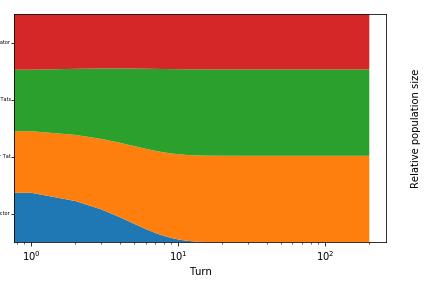
\includegraphics[width=.6\textwidth]{./assets/images/ecological_tournament.png}
    \caption{Results on an ecological tournament with Tit for Tat, Tit for Two Tats,
    Cooperator and Defector.}
    \label{fig:ecological_tournament}
\end{figure}

The process is then repeated for a given number of future tournaments.
Figure~\ref{fig:ecological_tournament} illustrates a simulation of our
ecological tournament, as shown strategies that cooperate quickly kill off the Defector.
A similar result was presented by Axelrod. In his ecological tournament cooperative
strategies managed to take over the population over time. On the other hand exploitative
strategies started to die off as weaker strategies were becoming extinct. In other
words they were dying because there was fewer and fewer prey for them to exploit.
In 1981, Axelrod also studied the prisoner's dilemma in an evolutionary context based
on the evolutionary approaches of John Maynard Smith~\cite{Smith1973,
Smith1974, Smith1979}. Smith is a well know evolutionary biologist as well
as an attendant of Axelord's second tournament. John Maynard Smith alongside George Price
are considered fundamental figures of evolutionary game theory. In~\cite{Smith1973}
they introduced the definition of an evolutionary stable strategy (ESS).

Imagine a population made up of individuals where everyone follows the
same strategy \(B\) and a single individual adopts a mutant strategy \(A\).
Strategy \(A\) is said to invade strategy \(B\) if the payoff of \(A\) against \(B\)
is greater than the expected payoff received by \(B\) against itself.
Since strategy \(B\) is in a population that interacts only with itself,
the concept of invasion is equivalent to a single mutant being able to outperform
the average population. Thus for a strategy to be ESS it must be able to resists
any invasion.

The work described in~\cite{axelrod1981}, studied the evolutionary stability of
Tit for Tat and although the strategy was likely to take over the population, its
stability was conditional on the importance of the future of the game. This is
represented by a discounting factor denoted as \(w\). Axelrod showed that if \(w\)
was sufficiently large, Tit for Tat could resist invasion by any other strategy.
Moreover, he showed how a small cluster of Tit for Tat players could invade a extortionate
environment.
Alongside the biologist William Donald Hamilton they wrote about the biological applications
of the evolutionary dynamics of the iterated prisoner's dilemma~\cite{Axelrod1984}
and won the Newcomb-Cleveland prize of the American Association for the Advancement
of Science. Arguing with Axelrod's results.
In~\cite{Boyd1987} Boyd and Lorderbaum show that if \(w\), the importance of the
future of the game, is large enough then no deterministic strategy is ESS because
it can always be invaded by any pair of other strategies. This was also independently
proven by~\cite{Pudaite1987}, so is reciprocity the answer to the emergence of
cooperation?

Cooperation can be favoured in several other settings, in~\cite{nowak1989},
Nowak and Sigmund studied the dynamics of the evolutionary
iterated prisoner's dilemma with a spectrum of stochastic strategies that only
remember their opponent's last move, not their own. They found that there can be
multiple fixed points that there can be an evolutionary stable coexistence among
multiple such strategies and in  1992,~\cite{Nowak1992b} explored how local
interaction alone can facilitate population wide
cooperation in a one shot prisoner's dilemma.

The two deterministic strategies Defector and Cooperator, were placed onto a two
dimensional square array where the individuals could interact only with the immediate
neighbours. The number of immediate neighbours could be either, fourth, six or eight.
As shown in Figure~\ref{fig:topologies}, where each node represents a player and
the edges denote whether two players will interact, this topology is refereed to
as spatial topology. Thus each cell of the lattice is occupied by a Cooperator
or a Defector.

\begin{itemize}
    \item At each generation step each cell owner interacts with its immediate neighbours.
    \item The score of each player is calculated as the sum of all the scores the player
    achieved at each generation.
    \item At the start of the next generation, each lattice
    cell is occupied by the player with the highest score among the previous owner
    and the immediate neighbours.
\end{itemize}

This topology is refereed to as spatial topology. The population dynamics of these
experiments were studied as a function of the temptation (\(T\)) payoff.
More specifically the following payoff matrix was used, which is equivalent
to equation~(\ref{eq:the_pd_payoffs}):

\begin{equation}
    \begin{pmatrix}
    R & S \\ T & P
    \end{pmatrix}
    =
    \begin{pmatrix}
        1 & 0 \\ b & 0
    \end{pmatrix}
\end{equation}

where \((b>1)\). Note that this representation fails constraint (\ref{eq:constrain_one}).

Local interactions proved that as long as small clusters of cooperators form and
they can benefit from interactions with other cooperators and while avoiding
interactions with defectors, global cooperation will continue.
Cooperation was also proven to be evolutionary beneficial under conditions were
the benefit to cost ratio \(\frac{b}{c}\) is higher to the number of neighbours
composed of unconditional cooperators and defectors~\cite{Ohtsuki2006} and
~\cite{MASUDA2003} showed that cooperation is more likely to emerge in a
small world topology. Moreover,~\cite{Perc2011}
studied graphs were a probability of rewiring ones connections was in place,
however, the rewire could be with any given node in the graphs and not just
with imitate neighbours. Perc etc all showed that ``making of new friends'' may
be an important activity for the successful evolution of cooperation,
but also that partners must be selected carefully and one should keep their number
limited.

\begin{figure}[!hbtp]
\centering
    \begin{subfigure}{.25\textwidth}
        \includestandalone[width=\textwidth]{assets/tex/square_lattice}
    \end{subfigure}
    \begin{subfigure}{.25\textwidth}\centering
        \includestandalone[width=\textwidth]{assets/tex/square_lattice_eight}
     \end{subfigure}
     \begin{subfigure}{.25\textwidth}\centering
        \includestandalone[width=\textwidth]{assets/tex/hexagonal_lattice}
     \end{subfigure}
     \caption{Spatial neighbourhoods}\label{fig:topologies}
    \end{figure}

Other mechanisms that have studied how cooperators may interact more so that
cooperation can emerge include reputation~\cite{janssen2006, nowak1998, suzuki2005}
and communication tokens~\cite{miller2002} which are partner identification methods.
Another related approach is using a tag based partner identification~\cite{choi2006,
hales2000, miller2002, riolo2001}. Tags allow cooperative strategies to distinguish
`them' from the rest.

This section has focused on evolutionary dynamics and how different evolutionary
settings can used to shed some light to how cooperation emerges in populations.
In the following section evolutionary settings are used to train strategies.

\subsection{Structured strategies and training}
\label{section:structured_strategies}

In Section~\ref{subsection:evolutionary_dynamics} several evolutionary
dynamic approaches used in the iterated prisoner's dilemma research were covered.
All of these approaches have a limitation, and that is their inability to develop
new strategies. In evolutionary settings strategies can learn to adapt their
actions over time based upon what has been effective and what has not. In
essence evolutionary reinforcement learning techniques can be used to train strategies for playing
the iterated prisoner's dilemma. A strategy must be represented in a generic strategy
archetype so it can be trained. Strategies that are discovered via strategy archetypes
are refereed to as structured strategies. This does not include only strategies
that have been trained, but any strategy that can emerge for any given structure
that covers a range of iterated prisoner's dilemma strategies. They are the opposite
to that of intelligent designed discussed in Section~\ref{subsection:intelligent_design}.
This section covers papers that proposed new structured strategies as well as
papers that explore new training algorithms are covered.

In Axelrod,~\cite{Axelrod1987} having realised the limitations of his evolutionary
work, decided to use reinforcement learning to demonstrated how to fine tune the
responses of an iterated prisoner's dilemma strategy and obtain a trained strategy.
The algorithm used in~\cite{Axelrod1987} was the genetic algorithm~\cite{Hoffmann1998}
and the structure was that of a lookup table. 
Axelrod decided to considered deterministic strategies that took into account
the last 3 turns of the game. For each turn there are 4 possible outcomes
\((CC, CD, DC, DD)\), thus for 3 turns there are a total of \(4\times4\times4=64\)
possible combinations. Therefore, the strategy can be defined by a series of
64 C's/D's, corresponding to each history; a lookup table.
A more generic lookup definition is a deterministic strategy which take into account
the last \(m\) actions.

In 1989~\cite{nowak1989}, Nowak and Sigmund proposed a structure for studying
sophisticated strategies instead of deterministic ones. They studied
a set of very simple strategies that remember only the previous
turn, and moreover, only record the move of the opponent. They are called reactive
strategies and they can be represented by using three parameters \((y, p_1, p_2)\), where \(y\) is the
probability to cooperate in the first move, and \(p_1\) and \(p_2\) the conditional probabilities
to cooperate, given that the opponent's last move was a cooperation or a defection.
Using the above notation a strategy can now be defined by a triple. For example,
Defector: (0, 0, 0), Cooperator: (1, 1, 1), Tit for Tat: (1, 1, 0) and Pavlov: (0, 1, 1, 0).

This framework was used by the authors to study the evolution of a population
composed of 99 reactive strategies. The strategy that managed to take
over was \textbf{Generous Tit for Tat} which is given by the triplet \((1, 0, \frac{2}{3})\).
In~\cite{Nowak1990} the reactive strategies structure was expanded and a formal definition
of a \textbf{memory one strategy} was given for the first time.
Memory one strategies consider the entire history of
the previous turn to make a decision (thus reactive strategies are a subset of
memory one).

If only a single turn of the game is taken into account and depending on the
simultaneous moves of two players there are only four possible states that
players could possibly be in. These are \(CC, CD, DC\) and \(DD\). A memory one
strategy is denoted by the probabilities of cooperating after each of these states,
\( p = (p_1, p_2, p_3, p_4) \in\mathbb{R}_{[0,1]}^{4} \).
A match between two memory one players \(p\) and \(q\) can be modelled as a
stochastic process, where the players move from state to state. More specifically,
it can be modelled by the use of a Markov chain~\cite{gamerman2006markov},
which is described by a matrix \(M\).

\begin{equation}\label{eq:markov_matrix}
    M =
\begin{bmatrix}
    p_{1} q_{1} & p_{1} (- q_{1} + 1) & q_{1} (- p_{1} + 1) & (- p_{1} + 1) (- q_{1} + 1)
    \\
    p_{2} q_{3} & p_{2} (- q_{3} + 1) & q_{3} (- p_{2} + 1) & (- p_{2} + 1) (- q_{3} + 1)
    \\
    p_{3} q_{2} & p_{3} (- q_{2} + 1) & q_{2} (- p_{3} + 1) & (- p_{3} + 1) (- q_{2} + 1)
    \\
    p_{4} q_{4} & p_{4} (- q_{4} + 1) & q_{4} (- p_{4} + 1) & (- p_{4} + 1) (- q_{4} + 1)
    \\
\end{bmatrix}
\end{equation}

The players are assumed to move from each state until the system reaches a state
steady, let the steady states vector be denoted as \(\bar{v}\).
The utility of a player can be given by multiplying the steady states of
\(M\) by the payoffs of equation~(\ref{eq:the_pd_payoffs}). Thus~\cite{Nowak1990}
offered a mathematical framework to calculate the utility of two players without
actually simulating the game. The payoff of a player \(p\) can be obtained by,

\[s_p = \bar{v} \times \begin{pmatrix} R \\ S \\ T \\ P \end{pmatrix}\]

The family of memory one strategies have been proven rather useful in the terms
of exploring strategies. The most famous work of memory one strategies is that
of Press and Dyson~\cite{Press2012}.
In 2012,~\cite{Press2012} presented
a new set of strategies called \textbf{zero determinant (ZD)}. The ZD strategies
are memory one strategies that manage to force a linear relationship between their
score and that of the opponent. The payoffs of players \(p\) and \(q\) are denoted
as:

\begin{align*}
    s_p = v S_p \\
    s_q = v S_q
\end{align*}

where \(v\) is a vector of the steady states of matrix \(M\) and \(S_p\), \(S_q\)
are the equivalent payoff values of the players for each state \(CC, CD, DC, DD\).
Using linear algebra, Press and Dyson showed that the dot product of the stationary
distribution of \(v\) with any vector \(f\) can be expressed as a \(4\times 4\)
determinant. In which one column is \(f\), one column is entirely under the control
of player \(p\) and another column is entirely under the control of player \(q\).
This meant that either \(p\) or \(q\) could independently force the dot product
of \(v\) with some other chosen vector \(f\) to be zero by choosing their
strategy so as to make the column they control be proportional to \(f\).
In particular, by

\begin{equation}\label{eq:exortion}
    f = \alpha S_p + \beta S_q + \gamma
\end{equation}

any player can force a given linear relation to hold between the long-run scores
of both players. Press and Dyson's suggested that these extortionate strategies
are the dominant family of strategies and that memory does not benefit them,
thus it would not benefit any strategy.

The ZD strategies have attracted a lot of attention. It was stated that
``Press and Dyson have fundamentally changed the viewpoint on the Prisoner's
Dilemma''~\cite{Stewart2012} and as stated in~\cite{hilbe2015} the American
Mathematical Society's news section said that ``the world of game theory is currently on fire''.
In~\cite{Adami2013, Hilbe2013b, Hilbe2013, hilbe2015, KnightHGC17,
Lee2015, Stewart2012} they question the effectiveness of ZD strategies. In~\cite{Stewart2012},
they revealed a more generous set of ZDs the~\textbf{Generous ZD},~\cite{Adami2013}
showed that ZD strategies were not evolutionarily stable and
in~\cite{Lee2015}, the `memory of a strategy does not matter' statement was
questioned. A set of more complex strategies, strategies that take in account
the entire history set of the game, were trained and proven to be more stable than
ZD strategies.

Complex strategy can be explored by using different structures. In 1996,
two were introduced by~\cite{Harrald1996} and ~\cite{Miller1996}.
Harrald and Fogel~\cite{Harrald1996}, considered a neural network structure.
Their neural network used a memory length of 3 and the actions were encoded as
continuous values in \([-1, 1]\),
where 1 meant complete cooperation. The input nodes represented 3 previous steps
of the player and the opponent and there was a single hidden layer of \(N\) fully
connected nodes and an output node that produced values from the range \([-1, 1]\).
Same year~\cite{Miller1996} considered finite state automata.
The specific type of finite automata that were used were Moore machines~\cite{moore1956}.
Finite state machine consist of a set of internal states. One of these states
is the initial state of the machine. A machine also consists of transitions
arrows associated with the states. Each arrow is labelled with \(A/R\) where
\(A\) is the opponent's last action and \(R\) is the player's response.
\cite{Miller1996} used a genetic algorithm to train finite state machines in
environments with noise. His results showed that even a small difference in noise
(from 1\% to 3\%) significantly changed the characteristics of the
evolving strategies. Three machines described in his paper were \textbf{Punish Twice},
\textbf{Punish Once for Two Tats} and \textbf{Punish Twice and Wait}.


Arguably the most complex strategies that have been trained are these of~\cite{Knight2017, KnightHGC17}.
In~\cite{Knight2017, KnightHGC17} present several powerful strategies
created using training. In these
papers the authors used genetic algorithms and particle swarm optimisation
algorithms~\cite{suganthan1999}. Their selected structures included, lookerup tables,
finite state machines, artificial neural networks~\cite{yegnanarayana2009} and
hidden Markov models~\cite{eddy1996}.
Hidden Markov models, are a variant of a finite state machine that use probabilistic
transitions based on the prior round of play to other states and cooperate or
defect with various probabilities at each state.
Additionally a variant of a look up table is also presented called the lookerup
archetype. The lookerup archetype responses based on the opponent's first \(n_1\)
moves, the opponent's last \(m_1\) moves, and the players last \(m_2\) moves.
Taking into account the initial move of the opponent can give many insights.
For it is the only move a strategy is truly itself without being affected by
the other player. Finally, a new structure called the Gambler was also introduced,
which is a stochastic variant of the lookerup archetype.

The structured strategies were put up against a large number of strategies in
two following settings:

\begin{itemize}
    \item A Moran process, which is an evolutionary model of invasion and resistance across
    time during which high performing individuals are more likely to be replicated.
    \item A round robin tournament.
\end{itemize}

The authors made use of an open source package called Axelrod-Python
( paper describing it and it's capabilities was published in 2016~\cite{Knight2016}).
The package includes more than 200 implemented strategies, this includes most
the strategies covered in this review.
These experiments are, to the authors knowledge, the biggest ones done in the
field in terms of different strategies.
In~\cite{Knight2017}, they performed a standard tournament and a noisy tournament.
For the standard tournament the newly introduced trained
strategies outperform the strategies outperform all the strategies of intelligent
design.In the case of noise there is one particular strategy that has not seen much
attention in the literature called ``Desired Belief Strategy''~\cite{Au2006}.

The result of~\cite{KnightHGC17} show that the trained strategies evolve an ability
to recognise themselves by using a handshake. This characteristic of the strategies
was an important one because in a Moran process this recognition mechanism allowed these
strategies to resist invasion.

Training can return a series of strategies. Differentiating between strategies
is not always an easy task. It is not obvious looking at a finite state diagram
how a machine will behave, and many different machines, or neural networks can
represent the same strategy. For example Figure~\ref{fig:machine_tft} shows
two finite automata and both are a representation of Tit for Tat.

\begin{figure}[!hbtp]
    \centering
    \includestandalone[height=.15\textheight]{./assets/tex/tit_for_tat_fsm}
    \caption{Finite state machine representations of Tit for Tat.}\label{fig:machine_tft}
\end{figure}

In order to distinguish the strategies and assuring that they are indeed
different~\cite{Ashlock2005} introduced a method called fingerprinting.
The method of fingerprinting is a technique for generating a functional signature for a
strategy~\cite{Ashlock2008}. This is achieved by computing the score of a strategy
against a spectrum of opponents. The basic method is to play the strategy
against a probe strategy with varying noise parameters. In~\cite{Ashlock2005}
Tit for Tat is used as the probe strategy. Fingerprint functions
can then be compared to allow for easier identification of similar strategies.
In Figure~\ref{fig:fingerprinting} an example of Pavlov's fingerprint is given.
Fingerprinting has been studied in depth in~\cite{Ashlock2008, Ashlock2009,
Ashlock2010, Ashlock2006a}.

\begin{figure}[!hbtp]
    \centering
    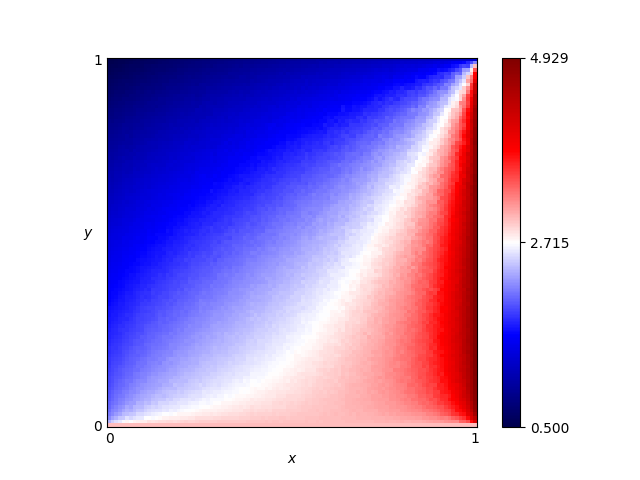
\includegraphics[height=.3\textheight]{./assets/images/Win-Stay_Lose-Shift.png}
    \caption{Pavlov fingerprinting with Tit for Tat used as the probe strategy.
    Figure was generated using~\cite{axelrodproject}.}
    \label{fig:fingerprinting}
\end{figure}

This section covered structured strategies and training methods. In the following
section software that has been developed with main aim simulating the iterated
prisoner's dilemma is presented.

\subsection{Software}\label{section:software}

The research of the iterated prisoner's dilemma heavily relays on software.
This is to be expected as the pioneer computer tournaments have become the main
mean of simulating the interactions in an iterated prisoner's dilemma game.
Many academics fields suffer from the lack of source code availability and the prisoner's dilemma
is not an exception. Though several of the tournaments that have been discussed so far were generated
using computer code not all of the source code was made available by the authors.
The code for Axelrod's original tournament is known to be lost and
moreover for the second tournament the only source code available is the code
for the 62 strategies (found on Axelrod's personal website~\cite{fortan_code}).

Several projects, however, are open, available and have been used as research
tools or educational platforms over the years. Two research tools are briefly mentioned
here~\cite{prison, axelrodproject} and two educational tools~\cite{pd_trust, pd_game}.
Both~\cite{prison, axelrodproject} are open source projects used as research
tools. PRISON is written in the programming language Java and preliminary version
was launched on 1998. It was used by it's authors in several publications, such
as~\cite{Beaufils1997} which introduced Gradual and~\cite{Beaufils1988}. The project
includes a good number of strategies from the literature but unfortunately the
last update of the project dates back in 2004.
Axelrod-Python is a package used by several papers covered in Section~\ref{section:structured_strategies}.
It is written in the programming language Python following best practice
approaches and contains the larger to date data set of strategies, known to the
author. The strategy
list of the project has been cited by publications~\cite{Anastassacos2018,
Hayes2017, Neumann2018} and the package has been for several manuscripts
such as~\cite{Goodman2018, Wang2017}.

The `Game of Trust'~\cite{pd_trust} is an on-line, graphical user interface
educational platform for learning the basics of game theory, the iterated prisoner's
dilemma and the notion of strategies. It attracted a lot of attention due to
being ``well-presented with scribble-y hand drawn characters''~\cite{trust_blogb}
and ``a whole heap of fun''~\cite{trust_bloga}. Finally~\cite{pd_game} is a
personal project written in PHP. It's graphical user interface platform that offers
a big collection of strategies and allows the user to try several matches and
tournament configurations.

\subsection{Conclusion and Contemporary period}\label{section:contemporary_period}

This section of the paper focused on reviewing articles that have been
published on the prisoner's dilemma. This review has partitioned the literature
into five different sections focusing on different aspects of the research.
Section~\ref{section:origin} covered the early years of research. This was when scientists
mainly grouped their students into pairs and asked them to simulate turns of
the game. An early figure discussed in the section was Rapoport. A brilliant
scientist that sought out the answer behind the emergence of cooperation and
introduced to the literature a number of successful strategies.

Following the early years the pioneer tournaments of Axelord were introduced
in Section~\ref{subsection:intelligent_design}. Axelrod's work offered the field
an exceptional agent based game theoretic framework to study the iterated prisoner's
dilemma. His original work asked researcher to develop their own intelligent
design of strategies, and the winning strategy of both his tournaments was the
Tit for Tat. The strategy however came with limitations which were explored by other
researchers and new strategies of intelligent design were introduced in order to surpass
Tit for Tat with some exceptional contributions such as Pavlov and Gradual.

Soon researchers came to realise that strategies should not just do well in a tournament setting
but should also be evolutionary robust. Evolutionary dynamics methods were
applied to many works in the fields, and factors under which cooperation
emerges were explored, as described in Section~\ref{subsection:evolutionary_dynamics}.
This was not done only for unstructured populations, where all strategies
in the population interacted with each other, but also in population where
interactions were limited to only strategies that were closed to each other.
In such topology it was proven that even in the one shot game cooperation can
indeed emerge.

Evolutionary approaches can offer many insights in the study of the prisoner's
dilemma. In evolutionary settings strategies can learn to adapt and take over
population by adjusting their actions; this has been referenced to as training.
Such algorithms can be applied so that evolutionary robust strategies can emerge.
Algorithms and structured used to train strategies in the literature were covered in
Section~\ref{section:structured_strategies}. Several strategies can emerge from
such processes, and to be able to differentiate between strategies fingerprinting
was introduced. The research of dominance and cooperation has been going on
since the 1950s, and several computer software have been developed along the way.
Few have been briefly discussed in Section~\ref{section:software}.

A large scale of articles has been covered in each of the corresponding sections
of this review. This literature doe not pretend to have covered all the publications
in the field. It will soon in the following section that the field has hab many
publications, exceeding 3000 articles. However, several important milestones
of the field have been presented here. In recent years the field is still active,
the game now serves as a model in a wide range of applications,
for example in medicine and the study of cancer cells~\cite{archetti2018, Kaznatchee2017},
as well as in social situations and how they can be driven by rewards~\cite{Dridi2018}.
A lot of work is still being published on  evolutionarily dynamics on graphs~\cite{Allen2017, hathcock2018, Liu2017}.
The study of the prisoner's dilemma is still an ongoing field of pioneer and innovating research,
where new variants and new structures of strategies are continuously being explored~\cite{Ohtsuki2018}.


\section{Analysing a large corpus of articles}\label{section:analysis}

\newpage
\bibliographystyle{plain}
\bibliography{bibliography.bib}
\end{document}